\section{Approach}
\label{sec:approach}
There are two steps in our approach: translation and revision.
Since both \pro and \con have the same triple form (node1, relation, node2), we do not differentiate their data structures later.

\subsection{Translation}
First, we translate the triple containing multi-word expressions (MWEs) on both sides directly, since MWEs are semantically less ambiguous than mono-words \cite{finlayson2011detecting}.
Specifically, we pack two nodes together as the final input. For example, given a triple, (``culture shock'', IsA, ``culture issue''), 
in order to give the translator a rich context, we first pack two nodes together into a  
contextual sentence with the comma separator (the comma is also always kept in the translation result, which is used for unpacking the translation result), such as ``culture shock, culture issue''.
Then, we put this contextual sentence into the translator.\footnote{Here, we use the API of Google translator \url{https://translate.google.com}.}
Last, we unpack the translated result by the comma separator to assemble the corresponding Chinese triple.
According to our statistics, triples with both MWEs account for 42\% and 11.6\% of total triples in \pro and \con, respectively.

\subsection{Revision}
%long tail semantic meaning
%the munition is a manner of the arm
%water well, well
%水井 井  5,230,000 7,380,000 
%the capital is at the proper noun
%capital  is distinct from low
%waterside isA bank
%
%beach    /r/RelatedTo    bank
%spring    /r/AtLocation   backseat of car
%
%great /r/RelatedTo well
%can /r/RelatedTo able
%spinach /r/RelatedTo can
%
%the mouse is at the feed mill
%the mouse is at the staple
%
%stray dog  /r/AtLocation   pound
%pound      /r/MannerOf    partition
%
%court /r/AtLocation park
%court /r/AtLocation gymnasium

Although the above approach can handle most cases, it cannot correctly translate some triples with intractable ambiguity, which usually use the long-tail semantic \cite{Tugwell20009} such as ``date'' in the triple (``date'', IsA, ``fruit''). 
%The reason may be that almost all present machine translation techniques, such as \cite{bahd2014neu,cho2014proper,suts2014sequ}, are essentially based on statistics, which means the decoder trained in the language model prefers outputting the sequence with a high co-occurrence frequency.\footnote{We hypothesize the training data has the similar distribution with the text data in web.}
%\begin{table}[!htbp]
%	\caption{Co-occurrence of Chinese word sense pair. (F) means wrong Chinese translation, which is also the translation of the machine translator, and (T) means correct translation. The number of co-occurrence reveals in the number of search result of Google Search Engine}
%	\label{tab:occur}
%	\begin{tabular}{|c|l|l|}\hline
%		English                                 & Translation & co-occurrence \\ \hline
%		\multirow{2}{*}{(date, fruit)/IsA}       & 时间, 水果(F)               & 191,000,000   \\ \cline{2-3} 
%		& 枣, 水果(T)                & 14,100,000    \\ \hline
%		\multirow{2}{*}{(can, shelf)/AtLocation} & 球, 舞厅(F)                & 3,310,000    \\ \cline{2-3} 
%		& 舞会, 舞厅(T)               & 1,480,000       \\ \hline
%	\end{tabular}
%\end{table}
%As shown in Table \ref{tab:occur}, ``时间'' occurs with ``水果'' more frequently than ``枣'' occurs with ``水果'', so the translator prefers translating ``date'' into ``时间'' incorrectly. It is the same to the translation of (``ball'', AtLocation, ``ballroom'') and some other triples. 

\begin{figure}[!htbp]
	\centering
	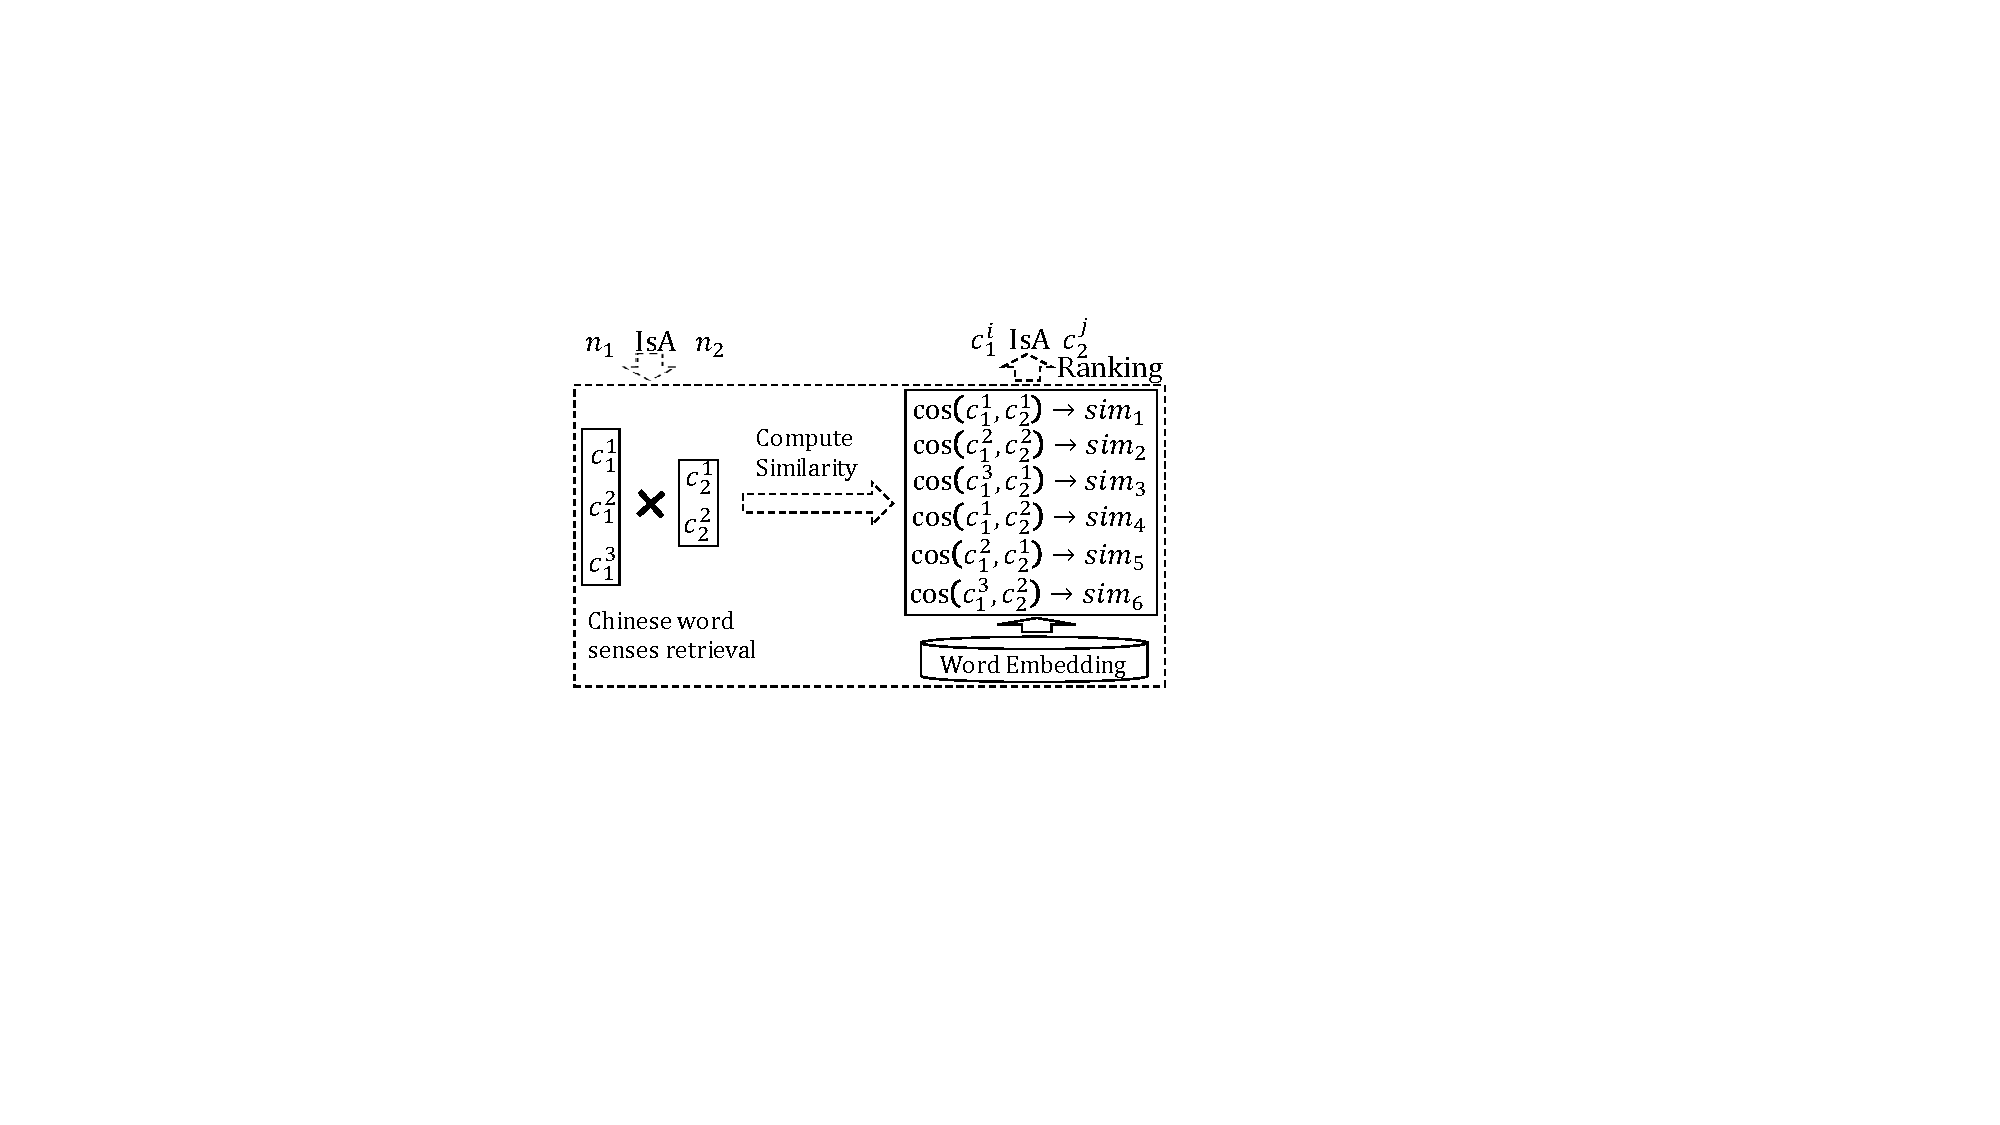
\includegraphics[width=\columnwidth]{figures/revision}
	\caption{Revision Step.}
	\label{fig:revision}
\end{figure}
Therefore, we take a further step to regard triples, containing at least one mono-word node, as the object to revise. 
Steps are shown in Figure \ref{fig:revision}. 
First, given one triple containing at least one mono-word node, such as (``date'', IsA, ``fruit''), 
we feed each node into the translator to look up all its Chinese word senses.
For the word ``fruit'', we can get all its Chinese word senses: ``水果'', ``果实'', ``果'', ``果类''. 
For the word ``date'', we can get all its Chinese word senses: ``日期'', ``约会'', ``枣''. 
%It doesn't matter even if we retrieve semantically duplicated Chinese word senses,
%because the translation with similar word senses will get close similarity, 
%and it has no effect on the subsequent ranking results.
Next, we obtain all the Chinese word sense combinations by a Cartesian product of all the possible Chinese word senses of the two nodes in the triple. It should be noticed that some MWEs may also have multiple Chinese word senses, but they usually produce tautological results, since they are less ambiguous as mentioned above, which does not affect the result.
Then, we calculate the similarities between every two Chinese word senses in each combination by word embedding.
Specifically, we segment every Chinese word sense into single Chinese words\footnote{Here, we use Jieba (https://github.com/fxsjy/jieba) to segment Chinese text.} and average their word embeddings as the embedding of the word sense, which is a well-accepted method for sentence embedding \cite{wieting2015towards,Shen2018}. 
Last, we rank the combinations of the Chinese word sense according to their similarities,
and select the most similar combination of Chinese word sense, such as (``枣'', ``水果''), as the final revised translation result.
